
\chapter{Introdução}

Informação de profundidade é uma das representações mais úteis para o entendimento de ambientes físicos \cite{lasinger2019towards} \cite{zhou2019does}. São também uma parte importante da caracterização de relações geométricas de uma determinada cena. As imagens de profundidades (ou mapas de profundidade) desempenham um papel importante em uma série de aplicações que envolvem visão computacional \cite{eigen2014depth}.  Entre elas, podemos citar: compreensão de cenas \cite{jaritz2018sparse}, veículos autônomos \cite{song2021self}, navegação de robôs \cite{ma2019sparse} navegação de VANTs, \cite{padhy2023monocular} fazendas inteligentes \cite{farkhani2019sparse}, e realidade aumentada \cite{du2020depthlab}. 

% \textit{Simultaneos Localization and Mapping} (SLAM) \cite{hu2012robust}

Os mapas de profundidade representam as distâncias de cada ponto (ou pixel) numa cena física em relação ao eixo do dispositivo de captura. Podem ser representados por imagens em escala de cinza, com as cores dos pixels sendo proporcionais à distância, com cinzas mais claros para objetos mais próximos e tons mais escuros para pontos mais afastados (e vice-versa), como exemplificado na Figura \ref{dmap}, que mostra uma cena em imagem RGB, seu mapa de profundidade e uma versão colorizada. Pontos cuja medição é desconhecida são representados por pixels totalmente pretos ou totalmente brancos \cite{dourado2020multi}.

\begin{figure}[h]
    \centering
    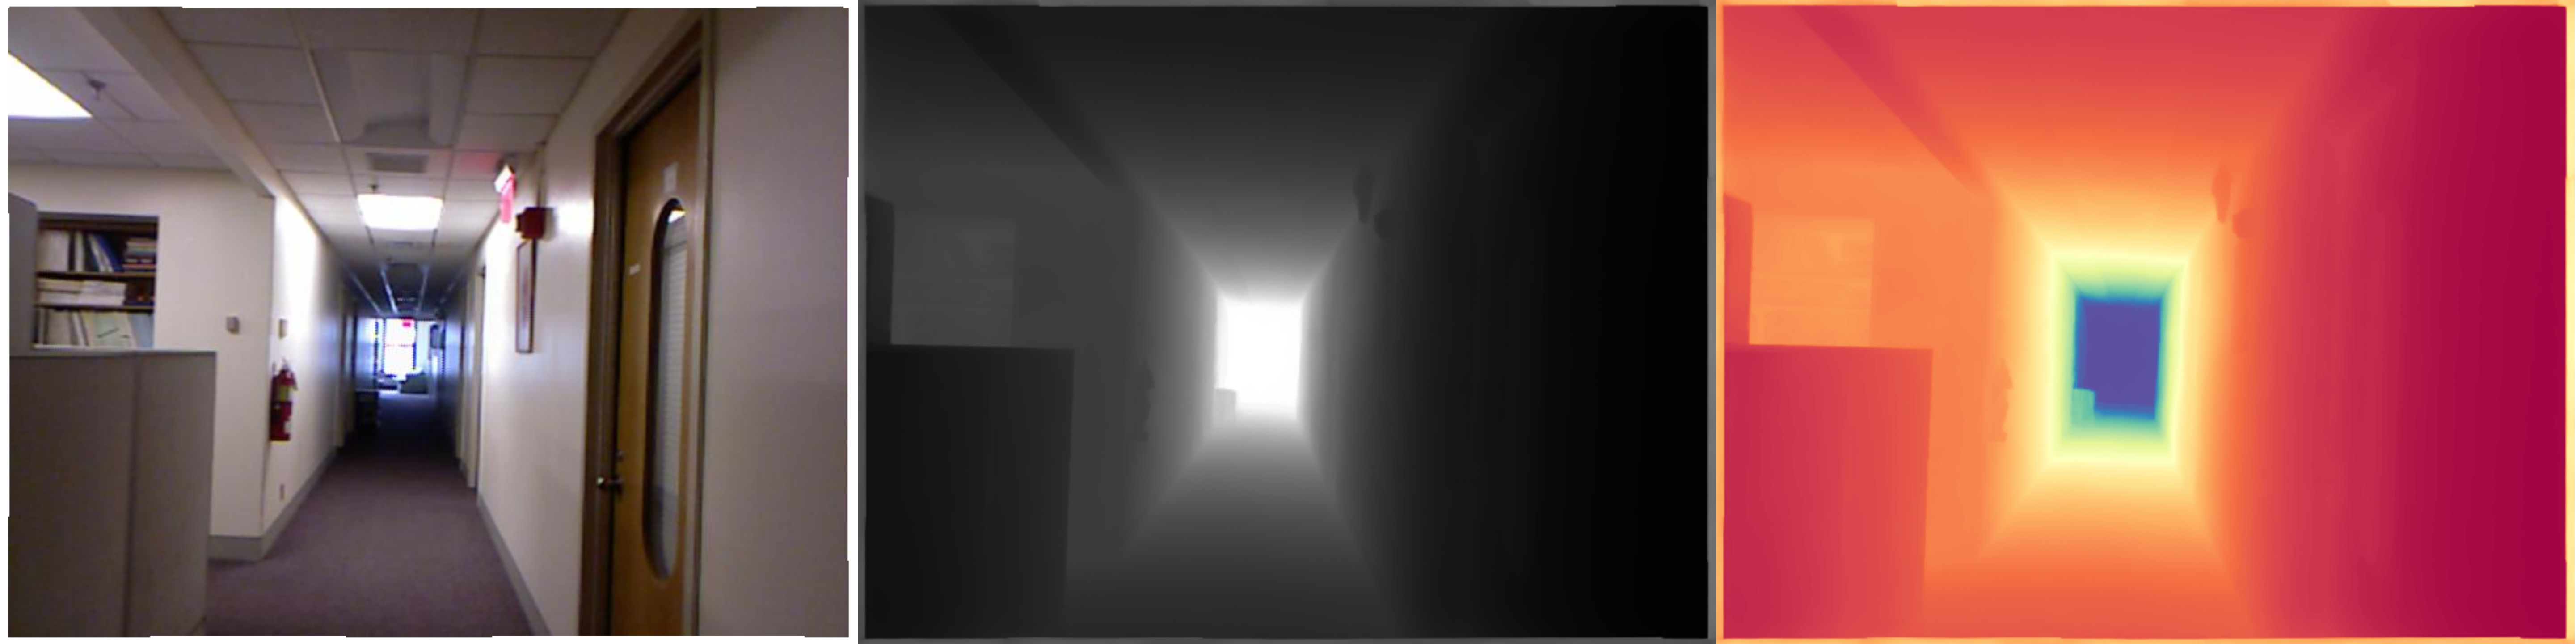
\includegraphics[width=\textwidth]{fig/example_depth.png}
    \caption{Exemplo de mapa de profundidade do \textit{dataset Nyu Depth V2}. No primeiro quadro, a imagem RGB, no segundo, o mapa de profundidade em escala de cinza, no terceiro uma colorização artificial para o mapa de profundidade.}
    \label{dmap}
\end{figure}


Para capturar tais imagens geralmente são empregadas câmeras RGB-D, que podem prover tanto informação de profundidade quanto imagens coloridas da cena. Entre suas tecnologias mais comuns, são encontrados diversos tipos de aquisição que podem ser baseados em visão estereoscópica, que trabalha com múltiplos ângulos de visão, sensores \textit{Time-of-Flight} (ToF) que emprega projeção de lasers infravermelhos (IR) estruturados e técnicas mais precisas como o LiDAR (\textit{Light Detection and Ranging}) \cite{castellano2023performance}.


Sensores de profundidade estão cada vez mais embarcados em equipamentos amplamente difundidos como dispositivos de realidade aumentada (Occulus, Kinnect) e até mesmo em smartphones \cite{du2020depthlab}, principalmente as câmeras ToF, pois são capazes de desempenhar de maneira satisfatória mesmo com baixa potência \cite{branscombe2018microsoft}. De acordo com \cite{xie2021ultradepth}, a adoção de sensores de profundidade em smartphones tende a aumentar nos próximos anos, com diversas aplicações como tradução de linguagem de sinais \cite{park2021enabling} e sistemas de navegação mobile para pessoas com deficiência visual \cite{see2022smartphone}.

%sinal 57, gestos 86, e aumentada 97

Ainda segundo \cite{castellano2023performance}, cada uma das técnicas de aquisição de imagens de profundidade possui lados negativos que podem impactar os dados. Por exemplo, as câmeras ToF podem sofrer com invalidação de pixels próximo a cantos ou bordas de objetos devido à interferências entre os raios IR em superfícies descontínuas ou reflexivas \cite{hansard2012time}, exemplificado na Figura \ref{errdepth}. Outros tipos de câmeras RGB-D mais comuns como o Microsoft Kinect ou Intel RealSense podem produzir valores inválidos em superfícies muito brilhantes ou reflexivas como espelhos, superfícies metálicas ou muito escuras \cite{zollhofer2019commodity}. Em ambientes internos, tais imagens podem conter até 50\% de dados faltantes. \cite{zhang2022indepth} \cite{zhang2018deep}. 

\begin{figure}
    \centering   
    \includegraphics[width=\textwidth]{fig/depth_problema.png}
    \caption{Exemplo de imagem RGB com mapa de profundidade apresentando leituras inválidas.}
    \label{errdepth}
\end{figure}

%problemas 27, 80, 98

Garantir a correta representação dos mapas em escala de pixel é de considerável importância para as tarefas que dependem de profundidade e que requerem um alto grau de segurança e confiabilidade dos dados, como veículos autônomos ou navegação de drones. A tecnologia LiDAR é a alternativa com implementação mais confiável entre as que foram citadas, no entanto, ressalta-se que nem o LiDAR e nem câmeras RGB-D convencionais produzem mapas completos e densos \cite{hu2012robust}. 

Ainda de acordo com \cite{hu2012robust}, o problema de preenchimento de valores indeterminados em mapas de profundidade depende inteiramente do sensor utilizado para sua captura. No caso do LiDAR, são produzidos mapas esparsos (approx. 95\% de esparsidade) e no caso de câmeras RGB-D ou câmeras ToF são produzidos mapas com partes faltantes em determinadas superfícies ou bordas. Os pixels inválidos normalmente são representados pelo valor 0 \cite{dourado2020multi}. De acordo com \cite{zhang2018deep}, o problema de correção de imagens de profundidade implica em fazer novas predições para áreas em que o sensor não retornou dados válidos.

Neste cenário, o presente trabalho apresenta uma abordagem baseada em técnicas de \textit{inpainting} utilizando redes neurais artificiais para realizar a correção de erros de mapas de profundidade capturados por câmeras RGB-D e sensores ToF.



% Neste cenário, tecnologias de aquisição e melhoramento dos dados foram amplamente pesquisadas pela ciência nos últimos anos. Recentemente foram exploradas técnicas que não dependem de sensores de profundidade, ou seja, que inferem a informação de profundidade a partir de uma única imagem RGB capturada a partir de uma câmera comum, essa abordagem é conhecida como \textit{Monocular Depth Estimation} (MDE). No entanto, métodos baseados em características puramente visuais   \cite{szeliski2022computer} \cite{hu2022deep}. 

     
	    
      


\section{Motivação} 

		

 
\section{Objetivos}


\subsection{Objetivo Geral}
Este trabalho possui como objetivo geral realizar a correção de mapas de profundidade com erros através de redes neurais artificiais e técnicas de \textit{inpainting}.

\subsection{Objetivos Específicos}

\begin{itemize}
    \item Realizar revisão de literatura de métodos de correção de mapas de profundidade.
    \item Escolher um método de \textit{inpainting} baseado em redes neurais artificiais.
    \item Estabelecer um método de geração de máscaras de erro para treinamento.
    \item Corrigir mapas de profundidade com algoritmo de \textit{inpainting} baseado em correção não-guiada.
    \item Corrigir mapas de profundidade com algoritmo de \textit{inpainting} baseado em correção guiada.
    \item Corrigir mapas de profundidade utilizando abordagem morfológica.
    \item Comparar as diferentes abordagens através de métricas de avaliação perante a diferentes níveis de pixels inválidos.
    
\end{itemize}

\chapter{Trabalhos Relacionados}

Em \citeonline{liu2012guided} é proposto um algoritmo de \textit{inpainting} para aprimorar os mapas de profundidade capturados com Kinect, estendendo o método original de marcha rápida (\textit{Fast Marching Method} - FMM) para reconstruir regiões desconhecidas incorporando uma imagem RGB alinhada como guia. Em seguida, um filtro de preservação de bordas é aplicado para reduzir o ruído nas regiões de separação de objetos. 

No trabalho de \citeonline{zhang2018deep}, foi desenvolvido um esquema que utiliza uma rede neural para inferir as normais de superfície e os limites de oclusão a partir de uma imagem RGB. Essas predições são combinadas com mapas de profundidade de câmeras RGB-D através de um método de otimização para computar a profundidade resultante de todos os pixels da imagem. A rede neural possui arquitetura totalmente convolucional utilizando a VGG-16 como \textit{backbone} e é treinada com as normais de superfície e limites de oclusão computados a partir da renderização de uma malha tridimensional reconstruída a partir de múltiplos ângulos de visão. 

\citeonline{dourado2020multi} introduz o método NSGA2CGP, uma abordagem de otimização multi-objetivo que integra programação cartesiana genética para otimizar filtros morfológicos em escala de cinza para completar mapas de profundidade utilizados em sistemas de navegação para pessoas com deficiência visual. O objetivo é minimizar tanto os erros quanto a complexidade dos elementos estruturantes dado as limitações energéticas dos sistemas de navegação embarcados. Além do erro, também foram mensurados na aplicação o consumo de energia e tempo de execução. 

\chapter{Marco Teórico}

\section{}



\chapter{Materiais e Métodos}

\subsection{Correção de mapas de profundidade} 

Para a tarefa de correção de mapas de profundidade utilizando redes neurais, o trabalho de \cite{hu2022deep} propôs duas categorias principais que se diferenciam pelos dados utilizados:

\begin{itemize}
    \item \textbf{Correção não-guiada} (Figura \ref{ung}): Objetiva completar diretamente as partes faltantes utilizando como entrada somente o mapa de profundidade.
    \item \textbf{Correção guiada} (Figura \ref{early} e \ref{late}): Objetiva completar as partes faltantes utilizando como entrada tanto o mapa de profundidade quanto a imagem RGB correspondente.
\end{itemize}

\begin{figure}[h]
    \centering
    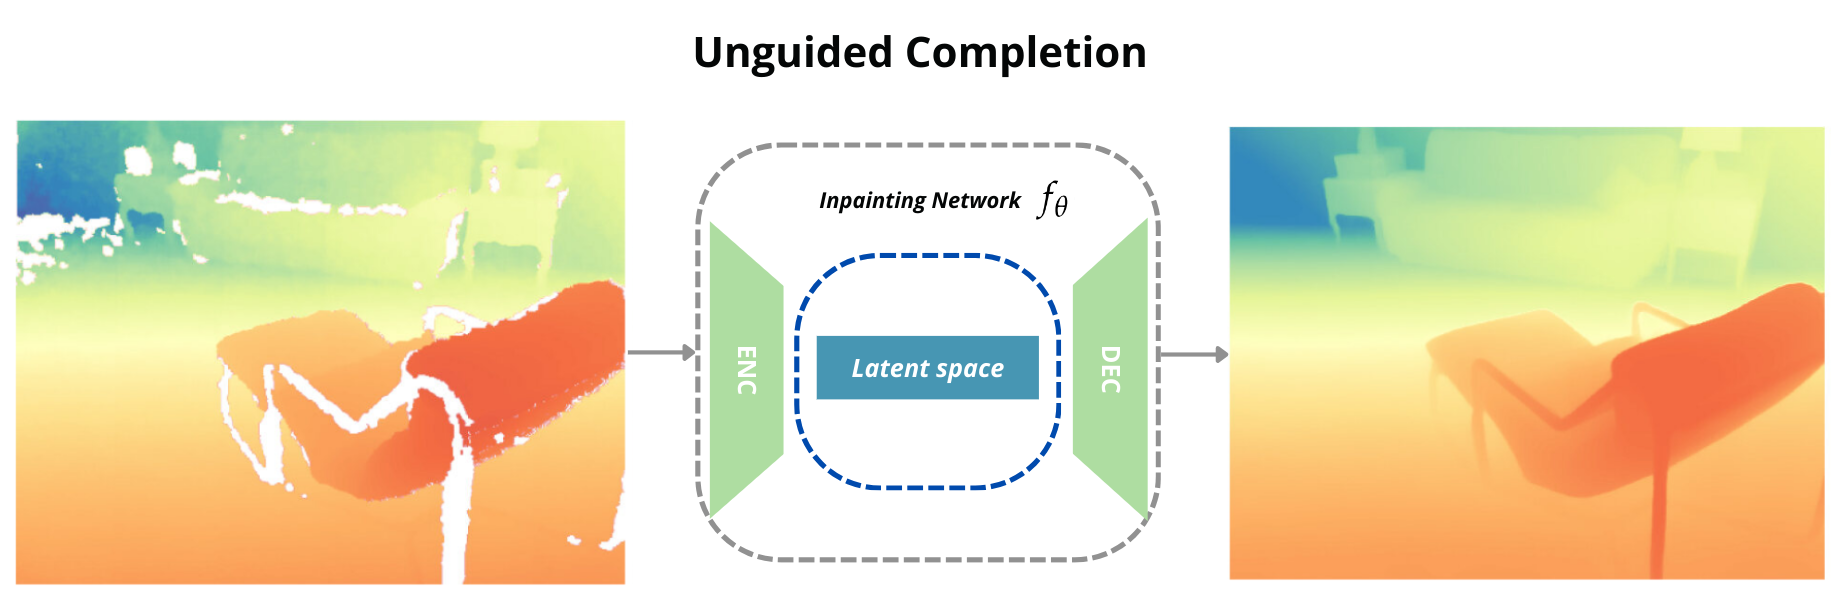
\includegraphics[width=\textwidth]{fig/unguided.png}
    \caption{Esquema de correção não-guiada.}
    \label{ung}
\end{figure}

A escolha da categoria de correção depende da quantidade de erros nas imagens. Quando há uma pequena quantidade de pixels inválidos, a correção não-guiada pode ser adequada, visto que não é necessário uma profunda extração de características dos dados. No entanto, no caso contrário, o uso de métodos guiados é indicado dado que existam grandes regiões com ausência de informação de profundidade ou que o mapa apresente uma grande esparsidade. Sendo necessário recorrer a extração dos atributos presentes na imagem RGB como bordas, contornos, estruturas de objetos não identificados pelo sensor e característica de descontinuidade de superfícies \cite{hu2022deep}.

Ainda no trabalho de \cite{hu2022deep}, nomeia-se outras subcategorias de técnicas de correção guiada. Uma delas é chamada de \textit{Early Fusion} (Figura \ref{early}) e consiste em utilizar a imagem RGB concatenada ao mapa de profundidade com erros como entrada da rede neural. Essa técnica possui a vantagem de ser simples e de baixa complexidade. A outra, conhecida como \textit{Late Fusion} (Figura \ref{late}) envolve transferir a fusão da imagem RGB com o mapa em ramos distintos da rede neural, chamados \textit{RGB Encoder-Decoder} e \textit{Depth Encoder-Decoder}.

\begin{figure}[h]
    \centering
    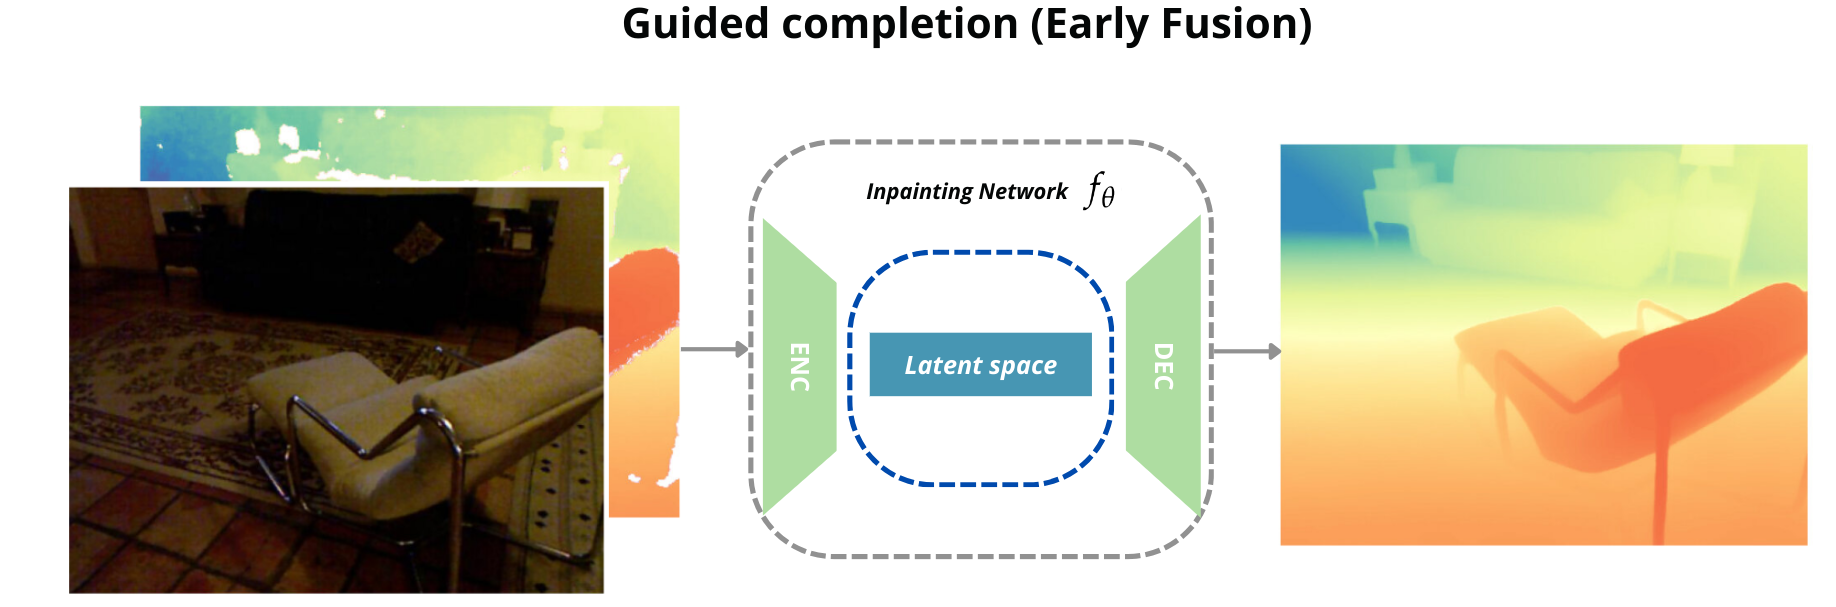
\includegraphics[width=\textwidth]{fig/earlyfusion.png}
    \caption{Esquema de correção guiada com \textit{Early Fusion}.}
    \label{early}
\end{figure}

\begin{figure}[h]
    \centering
    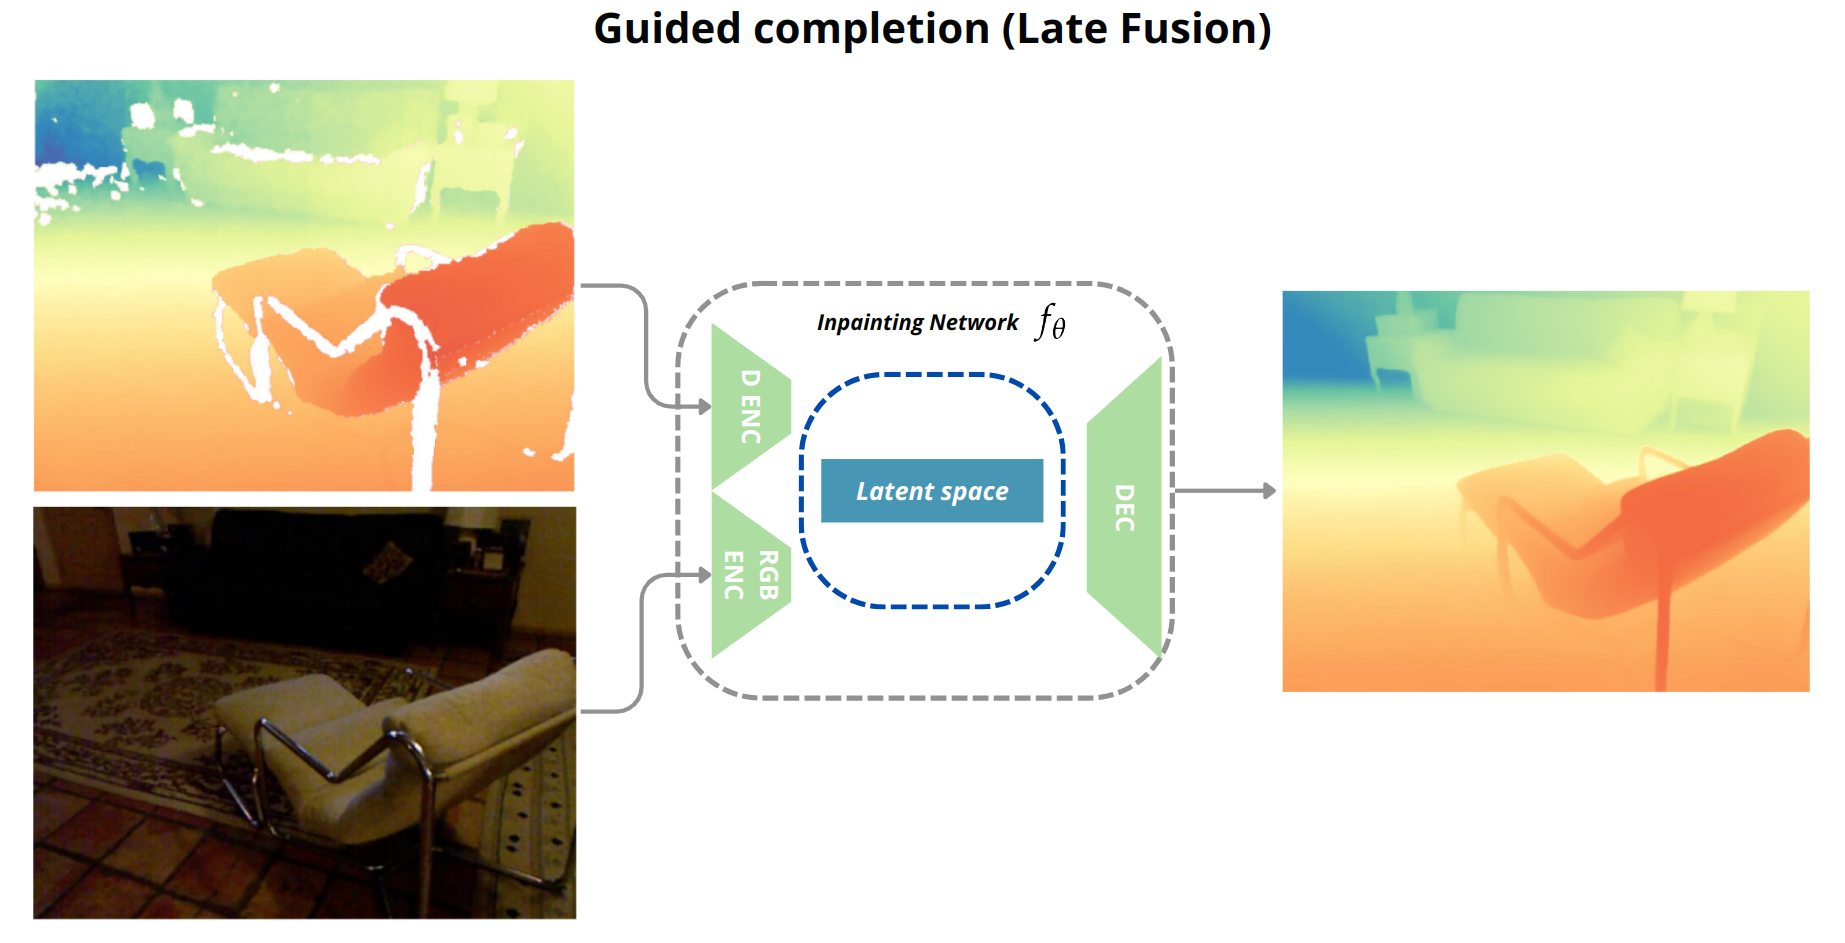
\includegraphics[width=\textwidth]{fig/latefusion.png}
    \caption{Esquema de correção guiada com \textit{Late Fusion}.}
    \label{late}
\end{figure}


\subsection{Large Mask Inpainting}

%Image inpainting is the process of completing or recovering the missing region in the image or removing some objects added to it. 

\textit{Image Inpainting} refere-se ao processo de recuperar regiões faltantes de uma imagem a partir de informação já existente \cite{elharrouss2020image}. Para sintetizar as partes indicadas, é necessário que haja o aprendizado da estrutura global da imagem, sendo imprescindível um vasto campo receptivo na rede neural. Dessa forma, é proposto por \cite{suvorov2022resolution} o sistema LaMa, \textit{Large Mask Inpainting} (Figura \ref{lama}), que é composto por elementos capazes de explorar o campo receptivo apropriado para essa tarefa, sendo eles: i) convoluções rápidas de Fourier (do inglês, \textit{Fast Fourier Convolutions}), ii) o uso de perda perceptual baseada em uma rede de segmentação e iii) uma estratégia de geração de máscaras para treinamento de alta cobertura.

\begin{figure}[h]
    \centering
    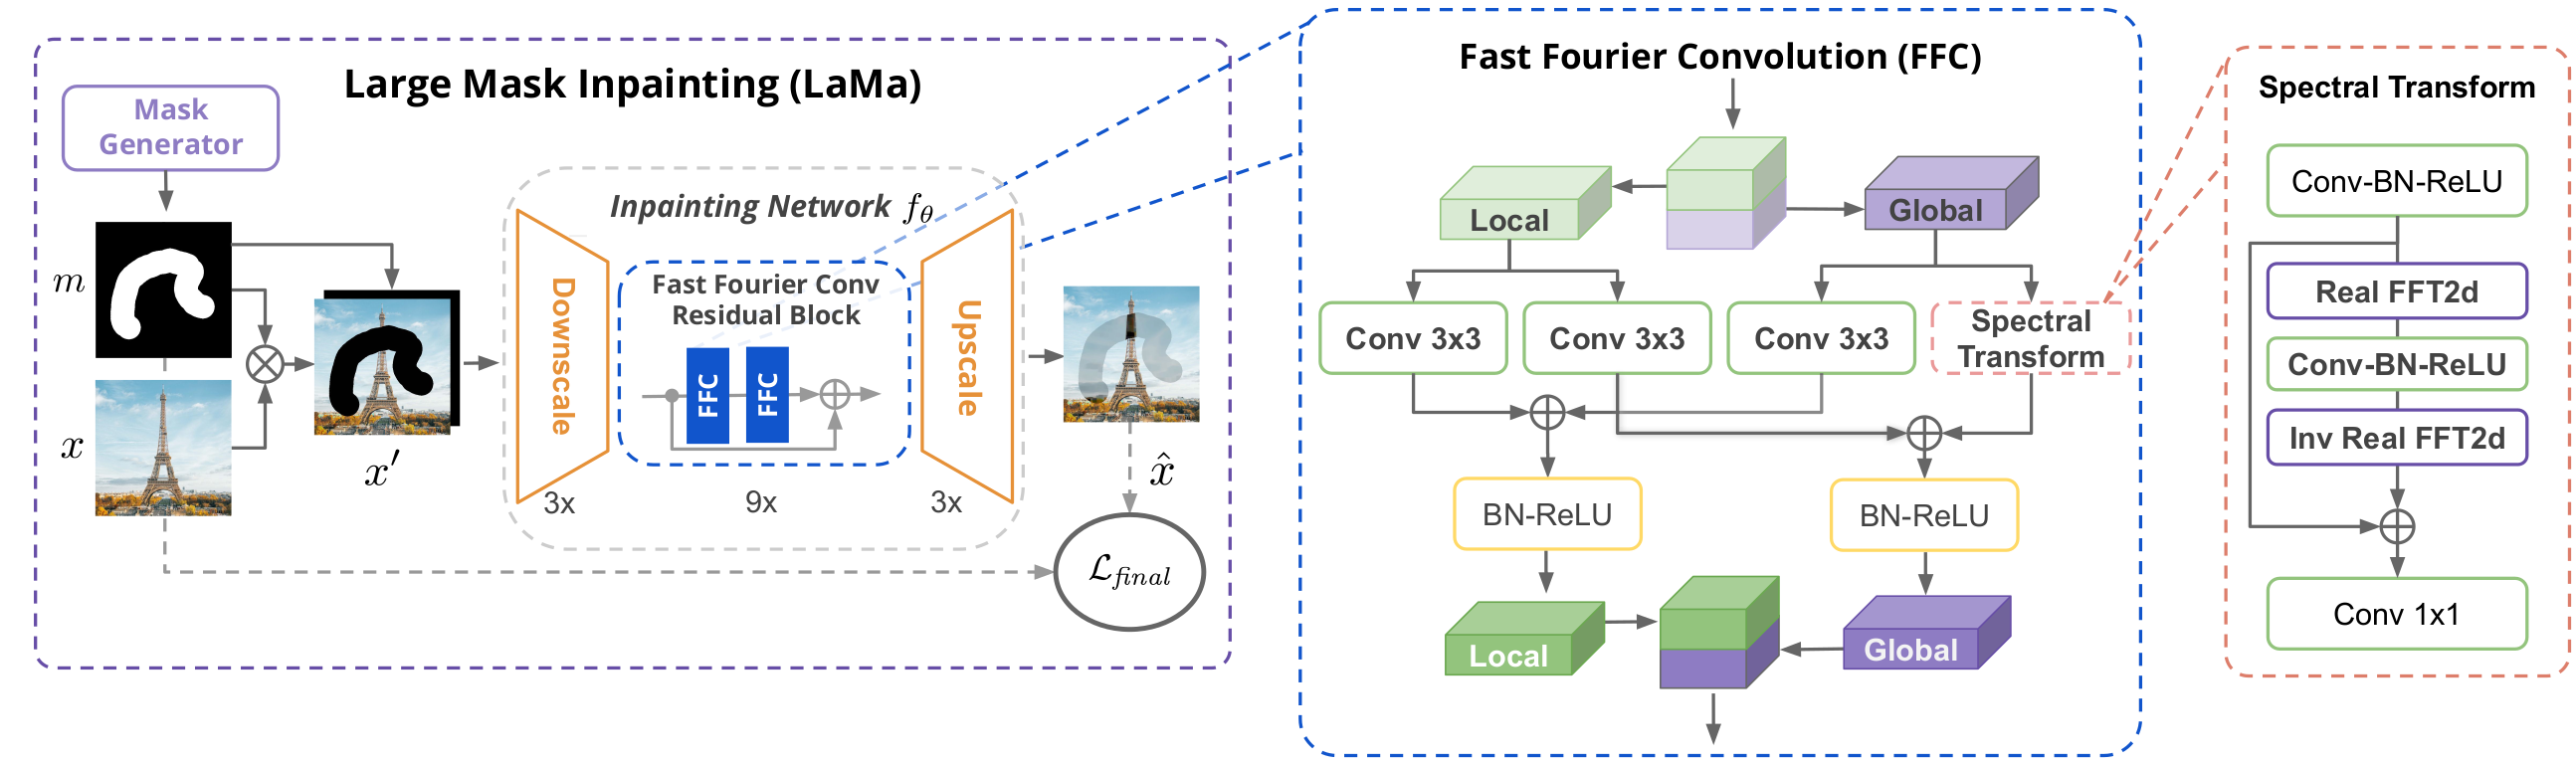
\includegraphics[width=\textwidth]{fig/lama.png}
    \caption{Esquema do método LaMa \cite{suvorov2022resolution}.}
    \label{lama}
\end{figure}

%explain receptive field?

\section{Datasets}

O presente trabalho exige um tipo de base de dados pouco encontrado na literatura, trios de imagem RGB, mapa de profundidade com erros e um outro mapa de profundidade denso e completo. De acordo com \cite{zhang2018deep}, uma das maneiras de se obter esses dados seria capturar imagens com uma câmera RGB-D de baixo custo e alinha-las com outra captura simultânea de um sensor mais preciso, porém essa abordagem é muito custosa, além de que não há disponibilidade de grandes conjuntos para treinamento.

O presente projeto pretende utilizar como base de dados principal o \textbf{Hypersim}. Um \textit{dataset} para compreensão de cenas baseado em cenas sintéticas fotorrealistas. Contendo 77.400 imagens de 461 cenas \textit{indoor} com pares de RGB e mapas de profundidade calculado deterministicamente, além de outras informações como normais de superfície, rótulos de segmentação e detecção de objetos e entre outros \cite{roberts2021hypersim}.

\section{Metodologia da Pesquisa}





\chapter{Resultados Preliminares}







